% courseword.tex 
% 
% MSc in High Performance Computing
%
% Programming Skills Coursework (in C++)
%
% Tim Beattie, David Canning, Marton Feigl, Max Sorantin
%

\title{Programming Skills Coursework}
\author{Tim Beattie, David Canning, Marton Feigl, Max Sorantin}
\date{\today}

%
% Preamble
%

\documentclass[12pt,a4paper]{article}

\usepackage{graphicx}
\usepackage[section]{placeins}
\usepackage{amsmath}
\usepackage{pdfpages}

%
% The following defines an environment for including source with syntax hilighting.
% (Copied from stackoverflow.com/questions/3175105/how-to-insert-code-%into-a-latex-doc) 
% Could be useful if we want to include source code in the report. 
%
% To use a different language, overwrite the language paramter in the code. I.e. write: 
%	\lstset{language=bash}
% before the beginning of the listing. 

% Then enter your code: 
%	\begin{lstlisting}
%		source code here ...
%	\end{lstlisting}
%

\usepackage{listings}
\usepackage{color}

\definecolor{dkgreen}{rgb}{0,0.6,0}
\definecolor{gray}{rgb}{0.5,0.5,0.5}
\definecolor{mauve}{rgb}{0.58,0,0.82}

\lstset{frame=tb,
  language=c++,
  aboveskip=3mm,
  belowskip=3mm,
  showstringspaces=false,
  columns=flexible,
  basicstyle={\small\ttfamily},
  numbers=none,
  numberstyle=\tiny\color{gray},
  keywordstyle=\color{blue},
  commentstyle=\color{dkgreen},
  stringstyle=\color{mauve},
  breaklines=true,
  breakatwhitespace=true,   
  tabsize=3
}


%Start of the Document Proper

\begin{document}

%Create Title Page
\maketitle
\newpage

%Number pages with Contents, Figure Table, etc. in Roman Numerals.
\pagenumbering{roman}

\tableofcontents
%\listoffigures 	
\newpage

%Begin normal page numbering from first section. 
\pagenumbering{arabic}



% Short Introduction
\section{Introduction}

Here is an example of what the C++ source would look like using the listing: 
 
\begin{lstlisting}
#include<iostream> 

int main (void)
{
	std::cout << "Hello, world!" << endl;

	return 0; 
}
\end{lstlisting}

Writing equations:  

\begin{equation} 
E_{tot} = m c^2 / \sqrt{1 - {v^2/c^2}}
\label{equation:chunktime}
\end{equation}

We can then refer back to equation \ref{equation:chunktime} like so. 




% How you planned your work
\section{Planning}
\label{Planning}
At the first meeting it was decided to set up version control, for details see sec.\ref{Revision Control}, and to create a Tasklist.
The latter was structured along the lines described in the "starting your project" section of the courserwork description and everyone
added specific tasks he could think of to the variouse sections and mark them as essential, i.e. needed for a basic implementation of the project, or polish.
After this Tasklist was established we agreed on a coding standard, build system and test framework, see sec.(\ref{Build Tools}) and sec.(\ref{Testing}), which was setup subsequentely.
It was than decided on the overall programm design/layout, see sec.(\ref{Design}), which led to the aim of writing the needed code/classes and their Unit Tests.
With the essential part of the Tasklist therefore implemented the focus was planned to be shifted to the "polish" tasks starting with profiling and optimisation (see sec.(\ref{Performance Tests and Analysis}).

However, in the real execution this was followed only up to the actual coding of the unit tests as profiling and optimisation was performed before carefull unit tests were in place. 




% Brief Summary of what tasks each member of the group did
\section{Assignment of tasks to group members}
\label{Assignment of tasks to group members}




% Description of your design
\section{Design}
\label{Design}



% Description of the programming language you used and how useful it was
\section{Programming Language}
\label{Programming Language}



% Description of the revision control ou used
\section{Revision Control}
\label{Revision Control}



% Description of the build tools you used and your views on the strengths and weaknesses of these
\section{Build Tools}
\label{Build Tools}



% Description of what testing you did and any test frameworks that were used
\section{Testing}
\label{Testing}

\subsection{Unit testing}
\label{unittesting}

The project's unit testing was done with UnitTest++, available at
\begin{center}
 http://unittest-cpp.sourceforge.net
\end{center}
Quote from this page:
\begin{center}
 \textit{"UnitTest++ is a lightweight unit testing framework for C++.  It was designed to do test-driven development on a wide variety of platforms. Simplicity, portability, speed, and small footprint are all very important aspects of UnitTest++."}
\end{center}

UnitTest++ was chosen because it was freely available, cross-platform, simple to set up and use, and equipped with a small but effective set of unit testing features. 
%Documentation for UnitTest++ can be found either on the UnitTest++ home page or in the following file in the project (once the project has been built):
%UnitTest++/docs/UnitTest++.html
\subsubsection{Implementation of the unittest framework}
UnitTest++ was downloaded as a .zip file and added to the project's Git repository in the "downloads" directory.
UnitTest++ was then integrated into the project's build system. Running "make test" in the project's top-level directory will unzip the downloaded file to the directory "UnitTest++", call UnitTest++'s makefile to build the UnitTest++ static library, run its self-tests and build plus run the project's unit tests which link in that library.
To ensure that the binary code being unit tested was the same code included in the popsim program, the project's build system was configured to build all C++ classes into a static library which was then linked into both the popsim program and the unit test program. This avoided problems which can occur when compiler or linker settings differ between multiple builds of the same source code.
The project's unit test program was implemented in a small C++ implementation file which provided main() and included test headers for the project's C++ classes.  Each class's test header contained one or more UnitTest++ "TEST" macros which implemented unit tests for that class.  The main() function simply contained a call to UnitTest::RunAllTests(). All test code was placed in the "test" directory.

\subsubsection{Unit tests for specific classes}
The project was begun with the firm intention of writing each class's unit tests during the development of that class, ensuring that every feature of every class would be robust and dependable before being used by the popsim program.  However, as the deadline approached, pressure was felt and several key classes were written without tests, with the intention to write tests later.
Due to this short comming, the team then lost considerable time on bug fixing, see sec.(\ref{Debugging}).
%a bug in the ordering of pixels in PPM and bitmask files and cells in the lanscape array: pixels in files were written by iterating over rows before columns, but elements in the array were being accessed by iterating over columns first, then rows.  The bug was present in several different classes, all of which did not yet have unit tests.
%The bug - and the loss of a day - could have been prevented by writing even basic unit tests of the affected classes before using them in the program.  Unit tests were then immediately written for all classes.
%


% Description of hw you did any debugging any any tools that were used       
\section{Debugging}
\label{Debugging}




% Description of what testing you did and any test frameworks that were usedi
\section{Performance Tests and Analysis}
\label{Performance Tests and Analysis}

Profiling runs were done using gprof on the CP Labs machines with an all-land 800x800 cell landscape for all runs of the program. To save time, timing runs were done on a faster machine (a core i7 laptop with a solid-state hard drive). 
For reference an initial run of the program was done and was found to take $47.437$ seconds.  Profiling the first implementation of the popsim program revealed that three functions accounted for approximately 80\% of the run time (see 1st profile in the shell output on next page).
The program spent more time in $Landscape::Update()$ than any other function. This was to be expected as all of the calculation was done there. However, one quarter of the run time was spent accessing elements of the landscape array, and this suggested a simple modification which improved performance significantly.
Namely, the removal of the bounds checking on every element access in $Array2D<T>::operator()$. This change was made and the profiling run was redone, producing the results int the 2nd profile.
Run time for this modified implementation was 27.123 seconds and therefore an improvement of 43\% over the implementation with bounds checking.
While bounds checking was included in the initial version of $Array2D<T>::operator()$ as a precaution, once the program had been demonstrated to work correctly, the considerable performance improvement achieved by removing it was considered to be worthwhile.
The reference documentation for class std::vector states that element access with bounds checking is provided by the function $std::vector<T>::at()$.  A timing run was performed with $std::vector<T>::operator[]$ replaced with $std::vector<T>::at()$, resulting in a run time of 35.127 seconds.
This was an improvement of 26\% over the initial implementation but still considerably slower than with no bounds checking at all.
All three options were left in the code in $Landscape::Update()$ with the unused options commented out.\\

A second optimisation became apparent on examination of the for loops in $Landscape::Update()$. The code was iterating over the x-coordinate of a cell, then over its y-coordinate.
While this was the intuitive order, it caused the code to stride through the array of cells by a distance proportional to the width of the landscape array instead of accessing the next cell in memory each time.
The order of the iterations was swapped, and another profiling plus timing led to the results in the 3rd profle. Run time with the order of iterations swapped was 12.366 seconds, a reduction of 54\% from the previous implementation and a reduction of 74\% from the original unoptimised implementation.\\

Finally, another optimisation was considered: making every landscape cell store pointers to its neighbours to the north, south, east, and west, so that function Landscape::Update() could access each cell's neighbours without calling Array2D::operator() four times.
Neighbours would be stored during initialisation of the array, meaning the array accesses would be done just once instead of once per update, reducing the number of memory accesses to non-local parts of the array. However, there was insufficient time for this change to be implemented and tested.

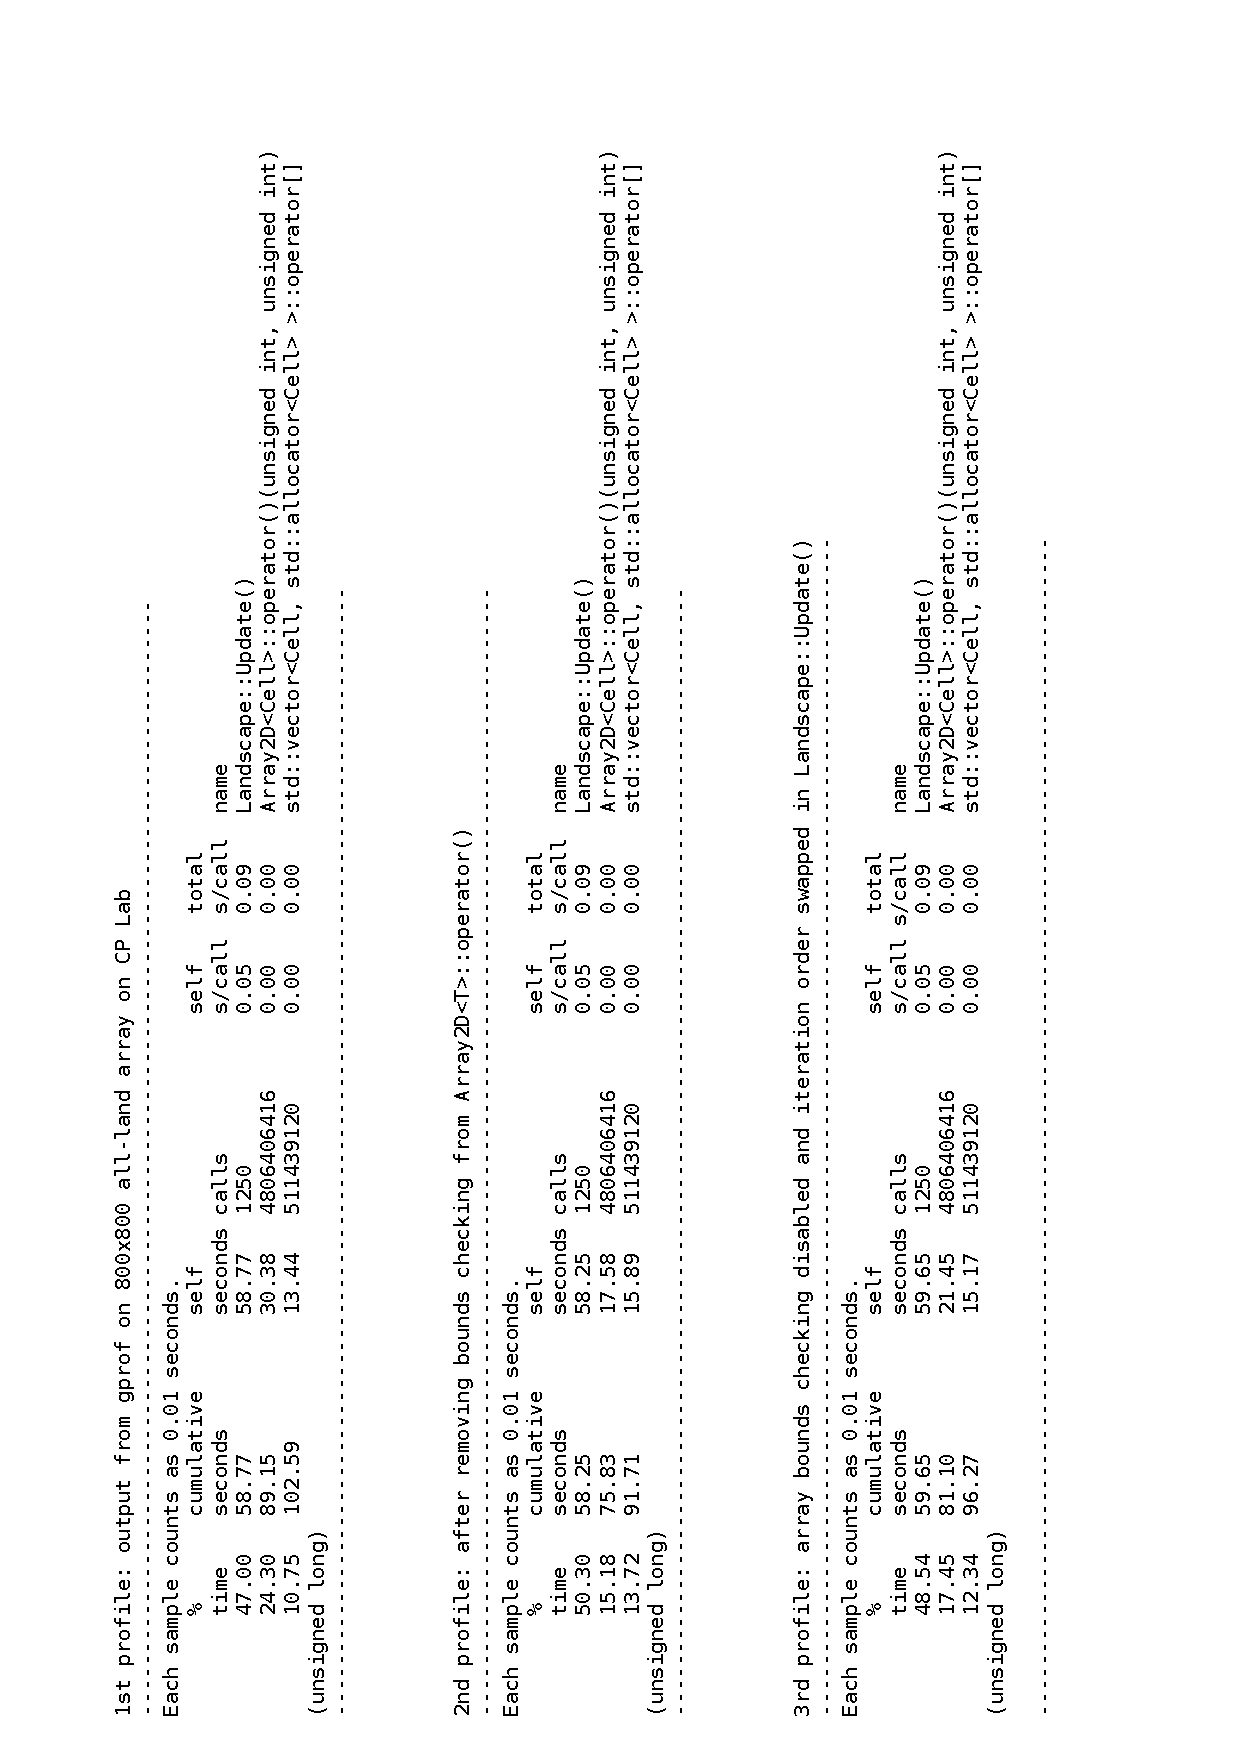
\includepdf[pages={1}]{Figures/profile2.pdf}



% Some brief conclusions 
\section{Conclusions}
\label{Conclusions}

Even thinking of unittests makes the design more split up and testable...



% Ideas for further work or what you would have done if you had more time.
\section{Further Work}
\label{Further Work}

\end{document}
